Consider a K-Dimensional pathfinding problem where no negative progress is allowed (similar to Unique Paths or Min Path Sum).
We can extend it to a K+1-Dimensional problem by simply considering a single new 'direction' in our calculation.
We have implemented this for Unique Paths in Figure \ref{fig:3d-unique-paths}.

We have shown that we can theoretically transform a K-dimensional pathfinding problem into a K+1-Dimensional pathfinding problem.
We can repeat this transformation N times in order to arrive at any N-Dimensional pathfinding problem.



\section{The Interstellar Problem Implementation Details}
Now that we have proved that The Interstellar Problem is solvable, we may attempt to implement a solution in Python.
This implemetation is tricky as we must simulate $n$ for loops where $n$ is the dimension count. The transformation from K to K+1-Dimensional pathfinding problems is trivial in theory, but requires thinking outside the box to implement in practice.
Numpy was used to 
access, store data in, and manipulate the input tensor as well as the $dp$ table.
This choice was made because Numpy allows us to access elements in n-rank tensors by providing a tuple of length $n$ as an index, rather than manually accessing each cell through a series of nested indices.
Numpy also allows us to easily initialialize n-rank tensors through the use of its $np.zeros(shape)$ function, rather than having to use something similar to Figure \ref{fig:zeros}:

\begin{figure}[H]
    \centering
    \begin{lstlisting}
    def initialize_array(dimensions):
        if len(dimensions) == 1:
            return [0] * dimensions[0]
        else:
            return [initialize_array(dimensions[1:]) for _ in range(dimensions[0])]
    \end{lstlisting}
    \caption{Example code to generate an n-rank tensor of zeros without Numpy}
    \label{fig:zeros}
\end{figure}

Numpy's $np.ndindex()$ is a function that provides an iterator yielding tuples of indices for a given shape.
It is particularly useful for iterating over the indices of n-dimensional arrays.
This function returns an object that can be iterated over, generating all possible index tuples for a specified shape.
\newpage
The pseudocode for The Interstellar Problem I is as follows:

\begin{enumerate}
    \item Initialize an n-dimensional array of zeros called $dp$ to store the number of paths for each cell, with $dp[R]$ set to 1.
    \item The $np.ndindex(shape)$ generates an iterator over all possible indices in the n-dimensional array.
    \item For each index, represented by the $current\_cell$:
    \item Iterate over each dimension using for $i$ in $range(num\_dimensions)$.
    \item Check if the current cell's index in the current dimension ($current\_cell[i]$) is greater than 0. If true, it means there is a valid cell to move from in that dimension.
    \item Create a copy of the current cell (denoted $prev\_cell$) and decrement the index in the current dimension ($prev\_cell[i] -= 1$). This represents the cell from which we are coming.
    \item Add the number of paths from the previous cell to the current cell in the $dp$ array ($dp[index] += dp[tuple(prev\_cell)]$).

\end{enumerate}

\section{Python Implementation of The Interstellar Problem 1}

Figure \ref{fig:nd-unique-paths} shows a Python Implementation of The Interstellar Problem I using the pseudocode described above.
The code is heavily commented so we can see the framework in action. Note that this approach can be trivially converted to calculate the Min Path Sum (The Interstellar Problem II) instead, or any other pathfinding problem through an N-dimensional field where negative progress is not allowed.

\begin{figure}[H]
    \centering
    \begin{lstlisting}
    import numpy as np

    def interstellar_1(dimensions):
        # Determine the number of dimensions
        num_dimensions = len(dimensions)
    
        # Initialize an n-dimensional array to store the number of paths for each cell
        shape = tuple(dimensions)
        dp = np.zeros(shape, dtype=int)
    
        # Set the number of paths for the starting cell to 1
        dp[(0,) * num_dimensions] = 1
    
        # Calculate the number of paths for each cell in the matrix
        for index in np.ndindex(shape):
            # Get the current index as an array
            current_cell = np.array(index)
            # Iterate over the array
            for i in range(num_dimensions):
                # If the current cell is not on the edge
                if current_cell[i] > 0:
                    # Add the previous cell's paths to the current cell [this happens from each valid direction in each dimension]
                    prev_cell = current_cell.copy()
                    prev_cell[i] -= 1
                    dp[index] += dp[tuple(prev_cell)]
    
        # The result is stored in the last cell of the matrix
        return dp[tuple(np.array(dimensions) - 1)]
    
    # Example usage:
    dimensions = (2,7,5)
    print(interstellar_1(dimensions))
    \end{lstlisting}
    \caption{Python Implementation of The Interstellar Problem I}
    \label{fig:nd-unique-paths}
\end{figure}

\subsection{Complexity Analysis of The Interstellar Problem I}
Let $n$ be the length of the tuple $dimensions$.
\begin{description}
    \item[Time Complexity:]
        The time complexity of filling a tensor of shape $dimensions$ with values,
        where each value is obtained through $n$ constant time additions is:\\$O((\prod_{i=1}^{n} dimensions_i) * n)$. This is because there are $\prod_{i=1}^{n} dimensions_i$ cells to fill, and each takes $n$ operations to complete, one addition from each dimension.
        
    \item[Space Complexity:] 
    The space complexity of filling a tensor of shape $dimensions$ with values,
    is $O(\prod_{i=1}^{n} dimensions_i)$.
    This is because there are $\prod_{i=1}^{n} dimensions_i$ cells to fill and store.
    
    \item[Overall:] Total:\\
        Time Complexity: $O((\prod_{i=1}^{n} dimensions_i) * n)$\\
        Space Complexity: $O(\prod_{i=1}^{n} dimensions_i)$

\end{description}

\subsection{Space Optimization of the Interstellar Problem}
Recall the two-row space optimization which was used for Longest Common Subsequence in Section \ref{subsec:lcs-optimized}.
Theoretically, this optimization can be applied to the Interstellar Problem, but instead of storing two rows of a 2D array,
we could store two ``slices'' of our input shape.
This is difficult to visualize in $>3$ dimensions, but it is possible for the following reason. As a ``slice'' of our input shape is being filled, it relies only on the previous ``slice'' of the shape.
If we set up the solution in such a way that we store only two ``slices'', we could eliminate the maximum value of $dimensions$ from the space complexity calculation.

A three dimensional visualization of the space optimized solution is shown in Figure \ref{fig:interstellar-optimization}.
For each iteration, the ``slice'' shown in blue is calculated from the ``slice'' shown in red. Notice that we only need to store the two colored slices at any point in time.

\begin{figure}[H]
    \centering
    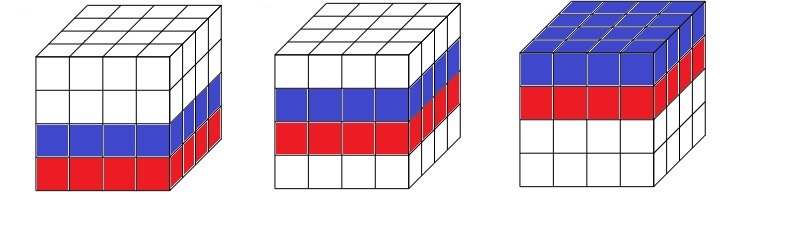
\includegraphics[width=0.8\linewidth]{visualization.jpg}
    \caption{Space Optimized Interstellar Problem Solution Visualized}
    \label{fig:interstellar-optimization}
\end{figure}